Bisherige temporale Lösungsansätze zur Steigerung der optisch wahrnehmbaren Qualität (siehe \ref{ch:Content1:subsec:Bisherige Temporalansätze})
lieferten gute Ergebnisse. Wir nehmen hier diesen Ansatz auf um den Algorithmus noch zeitlich stabiler zu machen.
\par

Allerdings: Um die \nameref{ch:Content2:sec:a Posteriori} Annahmen und die Vorbedingungen der Quantilfunktion \ref{eq:inverse Funktion}
für unseren Algorithmus zu erfüllen, brauchen wir eine erneute Permutation! Denn durch die Permutation haben wir wieder garantiert, 
dass je ein Anfangswert $x \in [0,1]$ auf je ein Pixelfarbwert abbgebildet wird.
Die Arbeit \cite[S.9/10]{hal02158423} motivierte diese Verbesserung. Da unser Algorithmus davon ausgeht, dass zwei aufeinanderfolgende Bilder gleiche Pixelwerte 
besitzen, erhoffen wir uns durch eine temporale Projektion ein Verbesserung bei der \nameref{ch:Content1:sec:blue noise} Verteilung 
falls sich z.B. durch Kamerabewegung die Farbgebung der Pixel zwischen Ihnen ändert. Die temporale Projektion, welche wir hier 
anwenden, baut auf aktuelle verbreitete Techniken des TAA auf \cite{INSIDETAA}.

\begin{figure}[H]
        \centering
        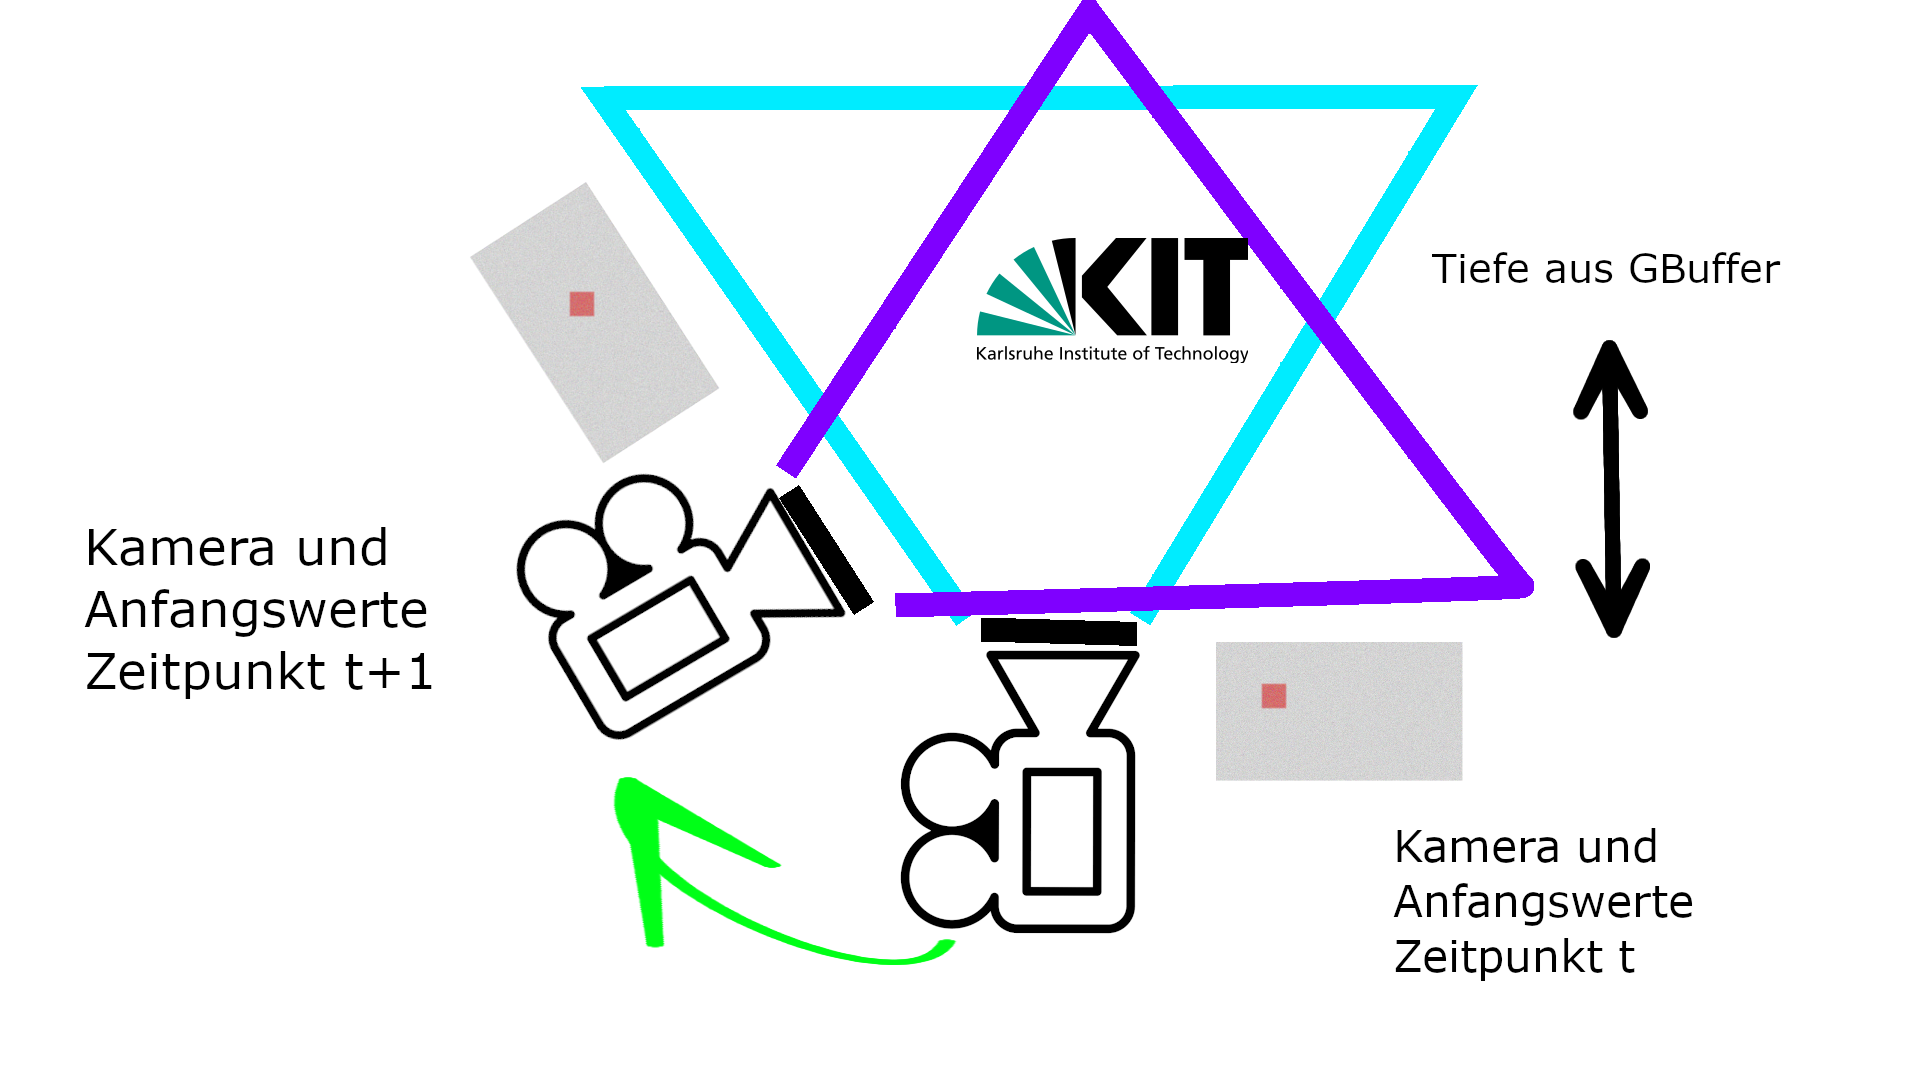
\includegraphics[width=\linewidth]{content/TemporalerAlg/Bilder/Reprojection/TemporalReprojectPrincipal.png}
        \caption{Übersicht temporales Projizieren}
        \label{pic:Uebersicht_Temporal_Reprojection}
\end{figure}

Wir benutzen die berechneten Tiefenwerte aus dem GBuffer (siehe auch unserer \nameref{pic:Render Graph}) und die jeweiligen 
View-Projektion-Matrizen der Kameras, um herauszufinden, welche Koordinaten der jeweilige Anfangswert von Bild t im Bild t+1 
haben würde aufgrund der Drehung.
\par 

Wir berechnen nun anhand der aktuell berechneten projizierten Position den jeweiligen Verschiebungsvektor jedes einzelnen 
Pixels und damit der neuen Position des jeweiligen Anfangswertes. Eine anschließende Mittelung über das gesamt Bild verschafft 
uns einen durchschnittlichen Bewegungsvektor. Dieser fließt nun in die Auswahl einer extra berechneten Retarget-Textur, die diese
Bewegung berücksichtigt. In einem zusätzlichen Vorberechnungsschritt wurden eine Vielzahl von Bewegungsvektoren auf die 
\nameref{ch:Content1:sec:blue noise} $Textur_{t}$ angewandt, bevor die Permutation zur $Textur_{t+1}$ berechnet und abgespeichert
wurde. Somit haben wir eine Vielzahl von neuen Retarget-Texturen geschaffen, die eine jeweilige zweidimensionale Verschiebung 
berücksichtigen.
\par 
Mit diesem Ansatz haben wir auch eine erneute Garantie einer Permutation, welche wir bereits bei dem \nameref{ch:Content2:sec:Retargeting}
erreicht haben.
%%%%%%%%%%%%%%%%%%%%%%%%%%%%%%%%%%%%%%%%%%%%%%%%%%%%%%%%%%%%%%%%%%%%%%%%%%%%%%%%%%%%%%%%%%%%%%%%%%%%%%
%%%%%%%%%%%%%%%%%%%%%%%%%%%%%%% comparrison retargeting + temporal reprojection 
%%%%%%%%%%%%%%%%%%%%%%%%%%%%%%%%%%%%%%%%%%%%%%%%%%%%%%%%%%%%%%%%%%%%%%%%%%%%%%%%%%%%%%%%%%%%%%%%%%%%%%
\newpage

  \begin{figure}[H]
    \begin{tcolorbox}
    \centering
    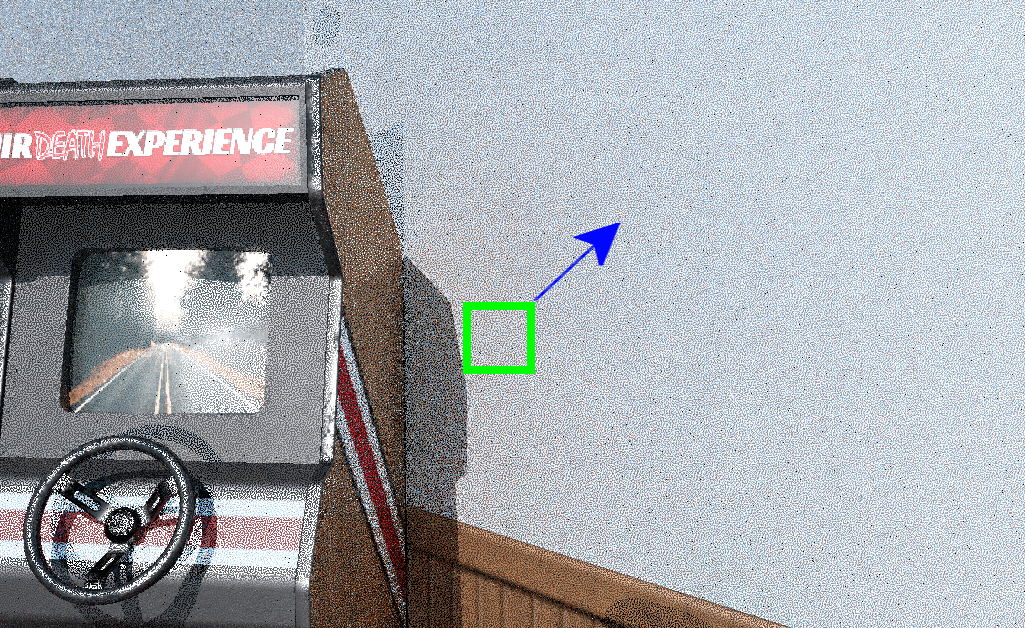
\includegraphics[width=0.5\linewidth]{content/TemporalerAlg/Bilder/Reprojection/Szene_bearbeitet.png}
    \end{tcolorbox}
    \caption{Ausschnitt(grüner Kasten) verfolgt bei Bewegungsvektor(blauer Pfeil)}
    \label{pic:TemporalReprComparison}
  \end{figure}


\begin{figure}[H]
  \begin{tcolorbox}[boxrule=4pt,sharp corners=downhill,title=Szene unter Kamerabewegung, fonttitle=\bfseries]
    %\begin{tcolorbox}[boxrule=4pt,sharp corners=downhill,title=Keine Projektion,colbacktitle=blue!50!white, coltitle=black]
    %\tcbsubtitle{Keine Projection}
    \paragraph{\hfill\colorbox{blue}{\textcolor{white}{nur Retargeting}}}
    %%%%%%%%%%%%%%%%%%%%%%%%%%%%%%%%%%%%%%%%%%%%%%%%%%%%%%%%%%%%%%%%%%%%%%%%%%%%%%%%%%%%%%%%%%%%%%%%%%%%%%
    %%%%%%%%%%%%%%%%%%%%%%%%%%%%%%% first row 
    %%%%%%%%%%%%%%%%%%%%%%%%%%%%%%%%%%%%%%%%%%%%%%%%%%%%%%%%%%%%%%%%%%%%%%%%%%%%%%%%%%%%%%%%%%%%%%%%%%%%%%
    \centering
    \begin{subfigure}[b]{0.2\linewidth}
      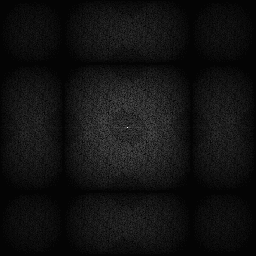
\includegraphics[width=\linewidth]{content/TemporalerAlg/Bilder/Reprojection/NoTemporalRepr/Ausschnitte/Ausschnitt1_FFT.png}
       \caption{FT}
       \label{pic:NoTemporalRepr_1_FFT}
    \end{subfigure}
    \begin{subfigure}[b]{0.2\linewidth}
      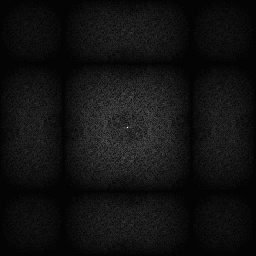
\includegraphics[width=\linewidth]{content/TemporalerAlg/Bilder/Reprojection/NoTemporalRepr/Ausschnitte/Ausschnitt2_FFT.png}
      \caption{FT}
      \label{pic:NoTemporalRepr_2_FFT}
    \end{subfigure}
    \begin{subfigure}[b]{0.2\linewidth}
      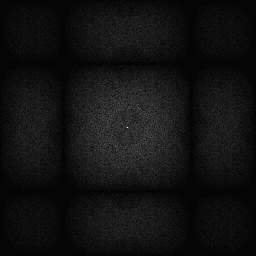
\includegraphics[width=\linewidth]{content/TemporalerAlg/Bilder/Reprojection/NoTemporalRepr/Ausschnitte/Ausschnitt3_FFT.png}
      \caption{FT}
      \label{pic:NoTemporalRepr_3_FFT}
    \end{subfigure}
    \begin{subfigure}[b]{0.2\linewidth}
        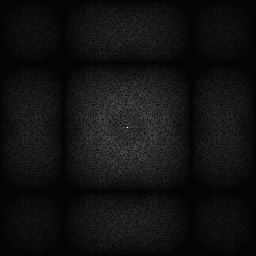
\includegraphics[width=\linewidth]{content/TemporalerAlg/Bilder/Reprojection/NoTemporalRepr/Ausschnitte/Ausschnitt4_FFT.png}
        \caption{FT}
        \label{pic:NoTemporalRepr_4_FFT}
    \end{subfigure}
    %%%%%%%%%%%%%%%%%%%%%%%%%%%%%%%%%%%%%%%%%%%%%%%%%%%%%%%%%%%%%%%%%%%%%%%%%%%%%%%%%%%%%%%%%%%%%%%%%%%%%%
    %%%%%%%%%%%%%%%%%%%%%%%%%%%%%%% second row
    %%%%%%%%%%%%%%%%%%%%%%%%%%%%%%%%%%%%%%%%%%%%%%%%%%%%%%%%%%%%%%%%%%%%%%%%%%%%%%%%%%%%%%%%%%%%%%%%%%%%%%
    \begin{subfigure}[b]{0.2\linewidth}
        
\includegraphics[width=\linewidth]{content/TemporalerAlg/Bilder/Reprojection/NoTemporalRepr/Ausschnitte/Ausschnitt1.png}
         \caption{}
         \label{pic:NoTemporalRepr_1}
    \end{subfigure}
    \begin{subfigure}[b]{0.2\linewidth}
        
\includegraphics[width=\linewidth]{content/TemporalerAlg/Bilder/Reprojection/NoTemporalRepr/Ausschnitte/Ausschnitt2.png}
         \caption{}
         \label{pic:NoTemporalRepr_2}
    \end{subfigure}
    \begin{subfigure}[b]{0.2\linewidth}
        
\includegraphics[width=\linewidth]{content/TemporalerAlg/Bilder/Reprojection/NoTemporalRepr/Ausschnitte/Ausschnitt3.png}
         \caption{}
         \label{pic:NoTemporalRepr_3}
    \end{subfigure}
    \begin{subfigure}[b]{0.2\linewidth}
        
\includegraphics[width=\linewidth]{content/TemporalerAlg/Bilder/Reprojection/NoTemporalRepr/Ausschnitte/Ausschnitt4.png}
         \caption{}
         \label{pic:NoTemporalRepr_4}
    \end{subfigure}
    %\end{tcolorbox}
    %%%%%%%%%%%%%%%%%%%%%%%%%%%%%%%%%%%%%%%%%%%%%%%%%%%%%%%%%%%%%%%%%%%%%%%%%%%%%%%%%%%%%%%%%%%%%%%%%%%%%%
    %%%%%%%%%%%%%%%%%%%%%%%%%%%%%%% third row 
    %%%%%%%%%%%%%%%%%%%%%%%%%%%%%%%%%%%%%%%%%%%%%%%%%%%%%%%%%%%%%%%%%%%%%%%%%%%%%%%%%%%%%%%%%%%%%%%%%%%%%%
    \tcblower
    %\begin{tcolorbox}[boxrule=4pt,sharp corners=downhill,title=Projektion,colbacktitle=green!50!white, coltitle=black]
    %\tcbsubtitle{Projection}
    \paragraph{\hfill\colorbox{blue}{\textcolor{white}{mit zusätzlichen temporalen Projizieren}}}
    \centering
    \begin{subfigure}[b]{0.2\linewidth}
      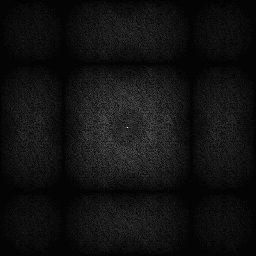
\includegraphics[width=\linewidth]{content/TemporalerAlg/Bilder/Reprojection/TemporalRepr/Ausschnitte/Ausschnitt1_FFT.png}
       \caption{FT}
       \label{pic:TemporalRepr_1_FFT}
    \end{subfigure}
    \begin{subfigure}[b]{0.2\linewidth}
      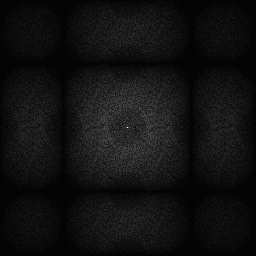
\includegraphics[width=\linewidth]{content/TemporalerAlg/Bilder/Reprojection/TemporalRepr/Ausschnitte/Ausschnitt2_FFT.png}
      \caption{FT}
      \label{pic:TemporalRepr_2_FFT}
    \end{subfigure}
    \begin{subfigure}[b]{0.2\linewidth}
      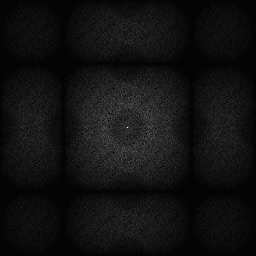
\includegraphics[width=\linewidth]{content/TemporalerAlg/Bilder/Reprojection/TemporalRepr/Ausschnitte/Ausschnitt3_FFT.png}
      \caption{FT}
      \label{pic:TemporalRepr_3_FFT}
    \end{subfigure}
    \begin{subfigure}[b]{0.2\linewidth}
        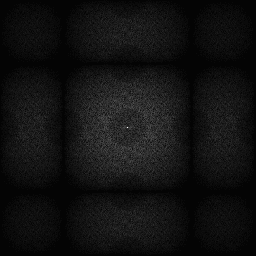
\includegraphics[width=\linewidth]{content/TemporalerAlg/Bilder/Reprojection/TemporalRepr/Ausschnitte/Ausschnitt4_FFT.png}
        \caption{FT}
        \label{pic:TemporalRepr_4_FFT}
    \end{subfigure}
    %%%%%%%%%%%%%%%%%%%%%%%%%%%%%%%%%%%%%%%%%%%%%%%%%%%%%%%%%%%%%%%%%%%%%%%%%%%%%%%%%%%%%%%%%%%%%%%%%%%%%%
    %%%%%%%%%%%%%%%%%%%%%%%%%%%%%%% 4th row
    %%%%%%%%%%%%%%%%%%%%%%%%%%%%%%%%%%%%%%%%%%%%%%%%%%%%%%%%%%%%%%%%%%%%%%%%%%%%%%%%%%%%%%%%%%%%%%%%%%%%%%
    \begin{subfigure}[b]{0.2\linewidth}
        
\includegraphics[width=\linewidth]{content/TemporalerAlg/Bilder/Reprojection/TemporalRepr/Ausschnitte/Ausschnitt1.png}
         \caption{}
         \label{pic:TemporalRepr_1}
    \end{subfigure}
    \begin{subfigure}[b]{0.2\linewidth}
        
\includegraphics[width=\linewidth]{content/TemporalerAlg/Bilder/Reprojection/TemporalRepr/Ausschnitte/Ausschnitt2.png}
         \caption{}
         \label{pic:TemporalRepr_2}
    \end{subfigure}
    \begin{subfigure}[b]{0.2\linewidth}
        
\includegraphics[width=\linewidth]{content/TemporalerAlg/Bilder/Reprojection/TemporalRepr/Ausschnitte/Ausschnitt3.png}
         \caption{}
         \label{pic:TemporalRepr_3}
    \end{subfigure}
    \begin{subfigure}[b]{0.2\linewidth}
        
\includegraphics[width=\linewidth]{content/TemporalerAlg/Bilder/Reprojection/TemporalRepr/Ausschnitte/Ausschnitt4.png}
         \caption{}
         \label{pic:TemporalRepr_4}
    \end{subfigure}
  %\end{tcolorbox}
  \end{tcolorbox}
    \caption{Erste beiden Reihen: kein temporales Projizieren; letzte beiden Reihen: Retargeting mit zusätzlichem temporalen Projizieren}
    \label{fig:Auswirkung temporales Projizieren}
\end{figure}

\begin{itemize}
  \item[nur Retargeting] Bei reinem \nameref{ch:Content2:sec:Retargeting} sieht man in der linken Hälfte des Ausschnitts Artefakte, die unsere 
                         \nameref{ch:Content1:sec:blue noise} Verteilung stören. Da zwischen den Bildern die Anfangswerte nicht projiziert
                         werden, nutzt die Bilderzeugung die anhand des vorherigen Bildes sortierten Anfangswerte. Die Sortierung allerdings
                         wurde an den vorherigen Pixelintensitäten gemacht. Da der Ausschnitt an einem inhomogenen Bildübergang gemacht wurde,
                         passen die neuen Pixelwerte nicht, um unsere \nameref{ch:Content2:sec:a Posteriori}(siehe Abschnitt \ref{ch:Content2:sec:a Posteriori})
                         Bedingung zu erfüllen. Die Anfangswerte wurden zuvor anhand völlig anderer Pixelwerte sortiert. 

  \item[Projizieren] Bei dem zusätzlichen Projizieren wird die Bewegung der Kamera auf die Anfangswerte mit angewandt. Somit erhalten wir auch in 
                      inhomogenen Bildübergängen gute Approximationen der Pixelwerte anhand der am vorherigen Bild sortierten Anfangswerte. 
\end{itemize}

